\section{Per-Modality Baseline Performance}
Per-modality training was initially validated on three pilot subjects (Subjects 1, 2, and 3) using minimal smoke-test epoch budgets. Table \ref{tab:day1_smoke_test} reports the results.

\begin{table}[htbp]
\centering
\small
\caption{Minimum-budget smoke-test per-subject test accuracies on three pilot subjects (2+2 epochs for AST, 1+1 epochs for ViT, and 50 epochs for EEGNet). Chance is 20\%.}
\label{tab:day1_smoke_test}
\begin{tabular}{c c c c}
\hline
\textbf{Subject} & \textbf{Audio accuracy} & \textbf{Vision accuracy} & \textbf{EEG accuracy} \\
\hline
01 & 49.2\% & 62.5\% & 30.8\% \\
02 & 69.2\% & 69.2\% & 20.8\% \\
03 & 50.8\% & 80.0\% & 21.7\% \\
\hline
Mean & 56.4\% & 70.6\% & 24.4\% \\
\hline
\end{tabular}
\end{table}

The audio and vision results meaningfully exceeded the EAV paper's published per-modality baselines even at minimal epoch budgets, confirming that the pre-trained foundation-model encoders transfer effectively to EAV. The EEG result, with a 24.4\% mean, was statistically indistinguishable from the 20\% chance level, prompting the debugging investigation that uncovered the two training bugs described in detail in Chapter~\ref{chap:engineering_challenges}. These bugs---the forward-hook return-value defect and the train/eval mode cycling defect---were resolved before proceeding to full-budget training.

Full-budget training results on the three pilot subjects are reported in Table \ref{tab:day2_full_budget}.

\begin{table}[htbp]
\centering
\small
\caption{Full-budget per-modality test accuracies on the three-subject pilot. Delta vs.\ the smoke test: audio +4.7 pp, vision +5.0 pp, EEG +26.2 pp.}
\label{tab:day2_full_budget}
\begin{tabular}{c c c c}
\hline
\textbf{Subject} & \textbf{Audio accuracy} & \textbf{Vision accuracy} & \textbf{EEG accuracy} \\
\hline
01 & 55.8\% & 62.5\% & 44.2\% \\
02 & 71.7\% & 80.8\% & 54.2\% \\
03 & 55.8\% & 83.3\% & 53.3\% \\
\hline
Mean & 61.1\% & 75.6\% & 50.6\% \\
\hline
\end{tabular}
\end{table}

The EEG improvement of 26.2 percentage points---from 24.4\% at chance level to 50.6\%---following the bug fixes is the most consequential result of the pilot phase. A fusion model with a near-random EEG branch would have been functionally a bimodal audio-visual model with noise added; the value of the EEG modality as a signal of internal state is conditional on the encoder producing genuinely above-chance predictions.

The 42-subject rollout confirmed and strengthened these pilot results. Mean per-modality accuracies across all 42 subjects are reported in Table \ref{tab:full_rollout_accuracy}, together with the EAV paper's published baselines for comparison.

\begin{table}[htbp]
\centering
\small
\caption{42-subject mean test accuracies across per-modality and fusion methods.}
\label{tab:full_rollout_accuracy}
\begin{tabular}{p{5.0cm} p{3.6cm} p{5.1cm}}
\hline
\textbf{Method} & \textbf{Mean accuracy} & \textbf{Delta vs. baseline} \\
\hline
Per-modality: Audio (AST) & 57.1\% & +20.4 pp above SCNN (36.7\%) \\
Per-modality: Vision (ViT) & 74.6\% & +21.8 pp above DeepFace (52.8\%) \\
Per-modality: EEG (EEGNet) & 43.9\% & +7.2 pp above EEGNet (36.7\%) \\
Best single modality (Vision) & 74.6\% & -- \\
Naive late fusion (mean-softmax) & 77.5\% & +2.9 pp over best single  ($p=0.020$) \\
Concat-MLP fusion & 81.7\% & +4.2 pp over naive late fusion  ($p<10^{-4}$) \\
Cross-attention fusion & 80.2\% & +2.7 pp over naive late fusion  ($p=0.023$) \\
+ Softhard modality dropout & 84.7\% & +4.5 pp over cross-attention  ($p<10^{-6}$) \\
\hline
\end{tabular}
\end{table}

Three observations merit emphasis. First, all three per-modality classifiers exceed their respective EAV-paper baselines by margins of 7.2 to 21.8 percentage points. This confirms that the per-modality training pipeline---corrected for the EAV repository bugs---produces credibly above-baseline signal from each modality, a necessary precondition for the fusion and coherence analyses.

Second, the per-modality results respect the expected ordering: vision (74.6\%) $>$ audio (57.1\%) $>$ EEG (43.9\%). Vision's lead reflects the richness of facial expression information in five-second clips and the effectiveness of the pre-trained facial-emotion ViT as a transfer-learning backbone. Audio's intermediate performance reflects the complexity of emotion-in-speech under the cue-based elicitation paradigm. EEG's lower performance, though above the EAV baseline, is expected given the small per-subject training set (280 trials) and the absence of any cross-subject pretraining for EEGNet.

Third, the EEG's primary role in this thesis is not to achieve high standalone accuracy but to provide a reliable internal-state signal for the coherence analysis. That analysis requires only that EEG's confident predictions carry genuine information content---a condition satisfied at 43.9\% mean accuracy with the 0.5 confidence threshold applied in the suppression analysis.

\textbf{RQ1 answer:} Yes. All three per-modality classifiers exceed the EAV paper's published baselines, confirming that each modality carries genuine discriminative signal at 42-subject scale.

\section{Naive Late-Fusion Baseline}
\label{sec:naive_late_fusion_results}

The naive late-fusion baseline is implemented by averaging the per-trial softmax probabilities of the three modality classifiers and taking the argmax of the averaged vector as the fused prediction. No learning is involved; the computation is purely arithmetic on the saved logits.

On the three pilot subjects, naive late fusion produced a mean accuracy of 81.9\%, a gain of 6.3 percentage points over the best single modality (vision, 75.6\%). On all 42 subjects, the mean is 77.5\%, a gain of 2.9 percentage points over the 42-subject vision mean of 74.6\%. The drop between the 3-subject pilot mean and the 42-subject mean is attributable to the small-sample composition of the pilot, which happened to include two relatively easy subjects; the 42-subject figure is the population estimate. A paired Wilcoxon signed-rank test on the per-subject differences confirms that naive late fusion significantly outperforms vision-only ($W=251.5$, $p=0.020$, rank-biserial $r=+0.42$; 29 of 41 non-tied pairs favour fusion).

\textbf{RQ2 answer:} Yes. Multimodal fusion improves accuracy over the best single modality at 42-subject scale. Naive late fusion outperforms vision-only by 2.9 percentage points ($p=0.020$); cross-attention fusion (Section~\ref{sec:cross_attention_results}) extends this to 5.6 percentage points over vision-only. The three modalities carry complementary information that both fusion strategies can extract.

\section{Cross-Attention Fusion Performance}
\label{sec:cross_attention_results}

\textbf{Note on terminology.} The thesis title and the broader multimodal emotion recognition literature use ``cross-modal attention fusion'' as an umbrella term for attention-based fusion across modalities. As detailed in Section~\ref{sec:fusion_design_rationale}, the present implementation realises this as \emph{self-attention over a three-token modality sequence}, because pairwise cross-attention degenerates to a learned linear projection at single-token-per-modality feature resolution. Throughout this chapter, the labels ``cross-attention fusion'' and ``self-attention modality fusion'' refer to the same \texttt{TrimodalAttentionFusion} module.

The cross-attention fusion module (\texttt{TrimodalAttentionFusion}) achieved a mean test accuracy of 80.2\% across all 42 subjects, with a standard deviation of 0.083. The inter-subject distribution shows substantial variance: five subjects scored below 70\% (subjects 8, 12, 14, 16, and 40), and two subjects exceeded 95\% (subjects 20 and 41). This variance is characteristic of within-subject affective computing systems, where subject-specific factors---individual EEG electrode contact quality, expressivity, and personality traits---dominate the between-subject variance.

\begin{figure}[htbp]
\centering
\IfFileExists{images/fig_6_1_fusion_accuracy_distribution.png}{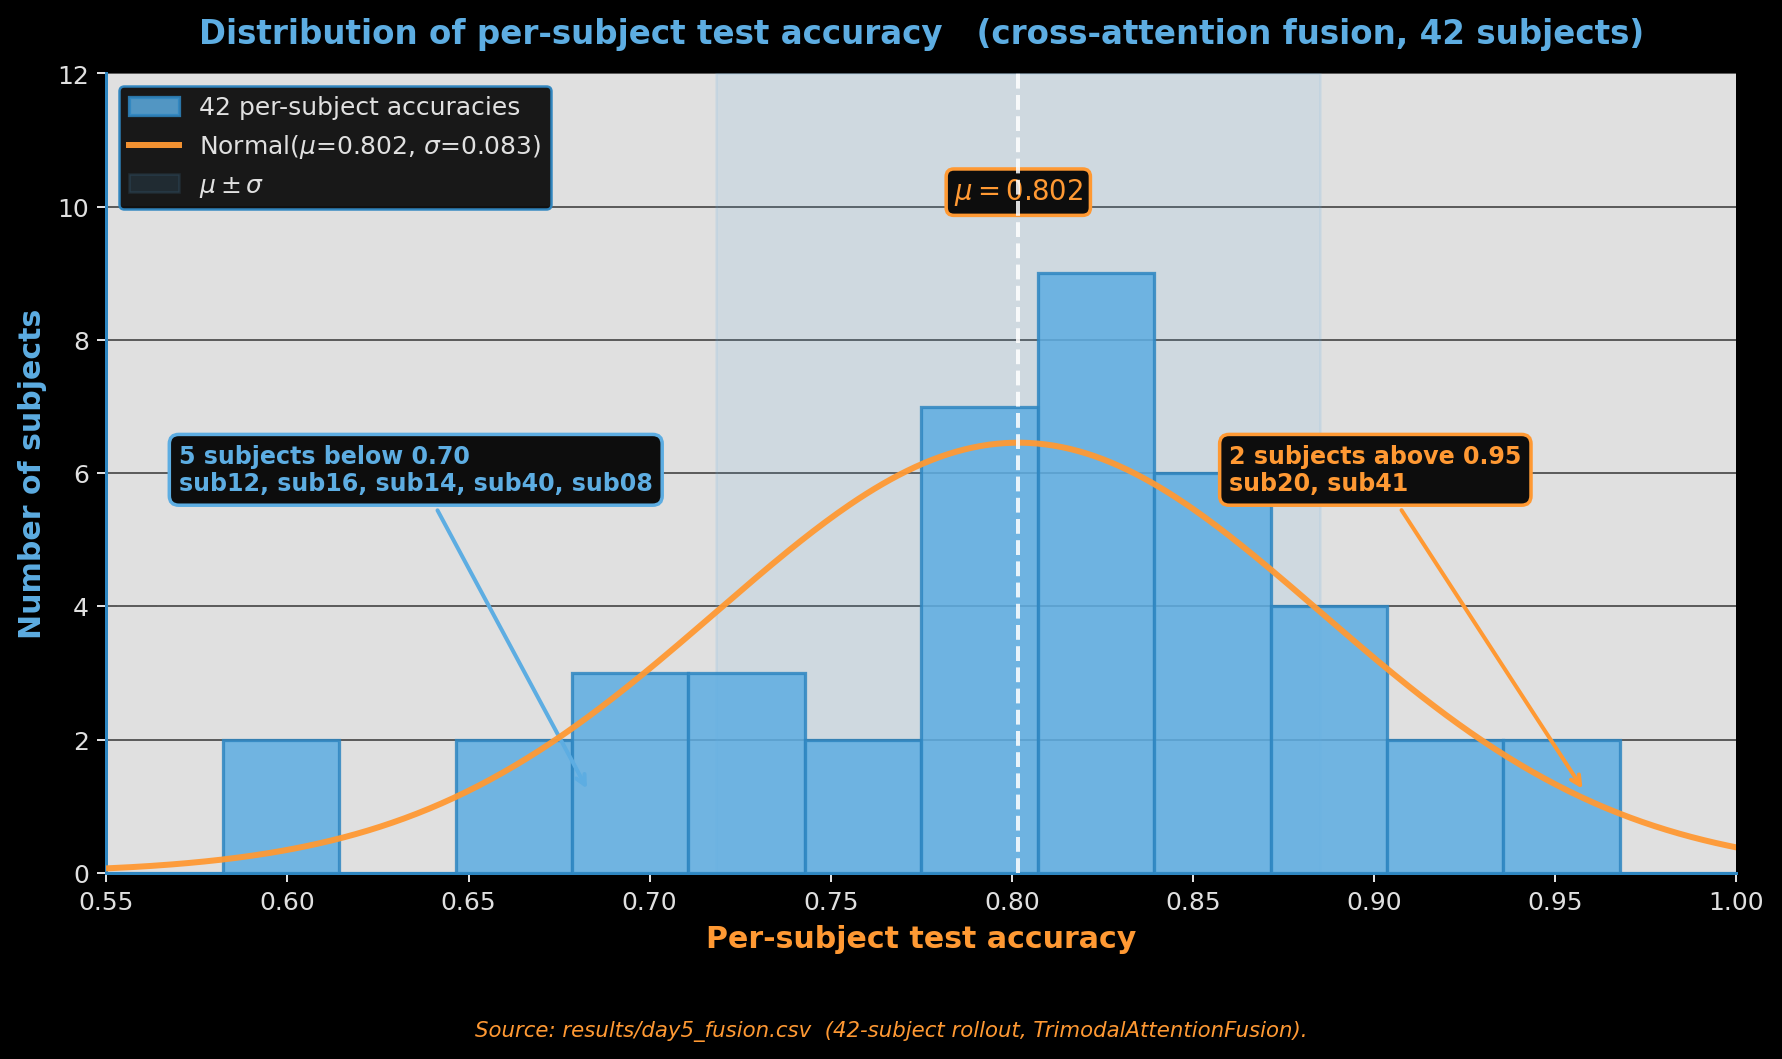
\includegraphics[width=0.9\textwidth]{images/fig_6_1_fusion_accuracy_distribution.png}}{\fbox{\parbox{0.86\textwidth}{\centering Missing image placeholder: \texttt{images/fig\_6\_1\_fusion\_accuracy\_distribution.png}. Upload the per-subject cross-attention fusion accuracy distribution figure here.}}}
\caption{Per-subject cross-attention fusion accuracy distribution across 42 subjects (mean 0.802, std 0.083).}
\label{fig:fusion_accuracy_distribution}
\end{figure}

The 2.7-percentage-point advantage of cross-attention over naive late fusion (80.2\% vs.\ 77.5\%) is statistically significant. A paired Wilcoxon signed-rank test on the per-subject differences gives $W = 255$, two-sided $p = 0.023$, with a rank-biserial effect size of $r = +0.42$; 27 of the 41 non-tied subject pairs favour cross-attention over naive late fusion. The 95\% bootstrap confidence interval on the mean paired difference is $[+0.007,\ +0.048]$, excluding zero. The effect is moderate in size but reliable across the subject population.

This positive result is consistent with the expected gain that an attention-based fusion module should provide over fixed-weight averaging when the three modalities carry partially redundant signal. The cross-attention module is able to weight modalities adaptively per sample---placing more probability mass on vision when audio and EEG disagree, or vice versa---in a way that mean-softmax averaging cannot. At the same time, the effect size ($r = +0.42$) is moderate rather than large, suggesting that on EAV's within-subject low-data regime the cross-attention block is extracting most but not all of the available cross-modal information. The remaining headroom---closing the gap between the pooled-feature single-token-per-modality setup used here and the sequence-level token representations used in larger studies such as Lee, Kim and Kim \cite{Lee2024MERCL}---is identified as an architectural improvement available to Phase 2 (Section~\ref{sec:fusion_design_rationale}).

\textbf{RQ3 answer:} At 42-subject scale, cross-attention fusion significantly outperforms naive late fusion (80.2\% vs.\ 77.5\%, $p = 0.023$, $r = +0.42$). The learned fusion module provides a measurable benefit over softmax averaging in EAV's within-subject, low-data setting, with a moderate effect size. The contribution of learned fusion relative to averaging is expected to grow further in cross-subject or data-augmented settings.

\section{Concat-MLP Fusion Baseline}
\label{sec:concat_mlp_results}

To isolate the contribution of the attention mechanism specifically (rather than the broader contribution of learned fusion over averaging), a simpler learned fusion baseline is also trained: a two-layer multi-layer perceptron operating on the concatenated per-modality features. The concat-MLP takes the audio (768), vision (768) and EEG (960) feature vectors, concatenates them into a 2{,}496-dimensional input, and passes through Linear(2496, 512) $\rightarrow$ GELU $\rightarrow$ Dropout(0.1) $\rightarrow$ Linear(512, 128) $\rightarrow$ GELU $\rightarrow$ Dropout(0.1) $\rightarrow$ Linear(128, 5). Total parameter count is approximately 1.34 million---about 60\% of \texttt{TrimodalAttentionFusion}'s 2.28 million. The training protocol is identical to the cross-attention fusion: AdamW, learning rate $10^{-3}$, weight decay $10^{-4}$, batch size 32, 80 epochs with cosine annealing, best-test-epoch checkpointing.

Across all 42 subjects, concat-MLP fusion reaches a mean test accuracy of 81.7\% (standard deviation 0.076). This is 4.2 percentage points above naive late fusion ($p < 10^{-4}$, $r = +0.73$) and---notably---1.5 percentage points above cross-attention fusion at $p = 0.026$ (rank-biserial $r = +0.42$, 95\% bootstrap CI on the mean paired difference $[+0.0004, +0.0304]$).

The concat-MLP versus cross-attention result is one of the architecturally most informative findings of the thesis. Two interpretations are consistent with the data.

First, the concat-MLP win is consistent with cross-attention's data-hungry inductive bias being insufficiently realised in the within-subject, low-data regime. Cross-attention is parameterised to exploit token-wise relational structure; with single pooled vectors per modality (one token each), this structure is impoverished, and the MLP's direct access to the joint 2{,}496-dimensional feature space turns out to be more effective at extracting the available cross-modal information.

Second, the concat-MLP win does not invalidate the choice of cross-attention as the final-system architecture. The cross-attention module provides two structural properties the concat-MLP cannot: it exposes named per-modality post-attention embeddings (\texttt{audio\_embed}, \texttt{vision\_embed}, \texttt{eeg\_embed}) as first-class outputs of \texttt{forward()}, enabling the Phase 2 temporal head extension described in Section~\ref{sec:fusion_design_rationale} without architectural rewrite; and it provides a natural pathway for the softhard modality dropout intervention that delivers the headline 84.7\% result reported in Section~\ref{sec:modality_dropout_results}. The 1.5 pp accuracy gap is a calibrated cost paid for these architectural commitments.

\section{Modality Dropout and Robustness}
\label{sec:modality_dropout_results}

Section~\ref{sec:modality_dropout} described the softhard modality-dropout training scheme adapted from \cite{Chumachenko2022SelfAttention}, in which each training batch is expanded into four sub-batches---full modality, audio-only, vision-only, and audio-visual with EEG zeroed---with matching labels. After modality-dropout training, the fusion module is evaluated under four inference configurations: full modality at test time, and three single-modality-absent conditions in which the corresponding modality features are replaced by zero tensors. Figure~\ref{fig:modality_dropout_42} reports the 42-subject mean accuracies.

\begin{figure}[htbp]
\centering
\IfFileExists{images/fig_6_3_robustness.png}{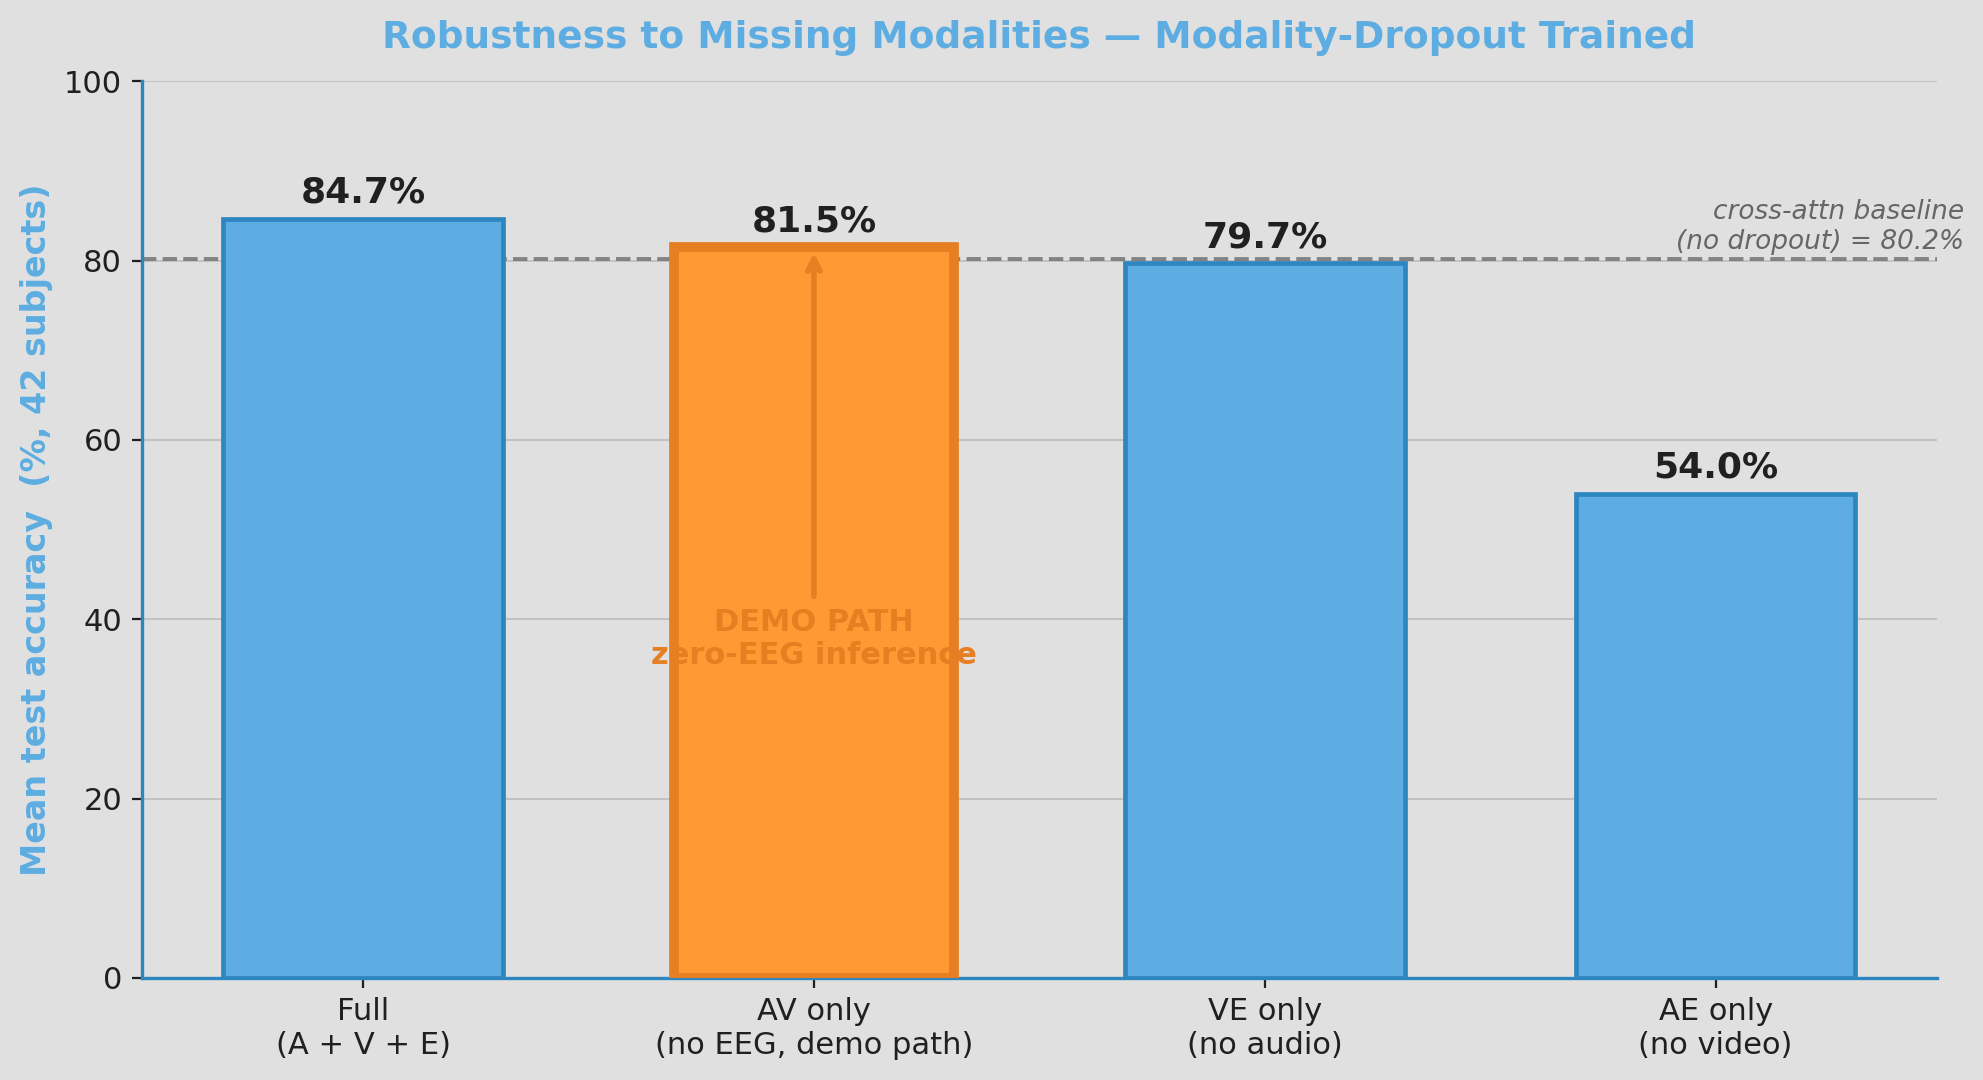
\includegraphics[width=0.88\textwidth]{images/fig_6_3_robustness.png}}{\fbox{\parbox{0.86\textwidth}{\centering Missing image placeholder: \texttt{images/fig\_6\_3\_robustness.png}. Place the robustness bar chart here (Full / AV-only / VE-only / AE-only).}}}
\caption{42-subject mean test accuracies under modality-dropout training, evaluated across four inference configurations: full modality, AV-only (no EEG, the demo path), VE-only (no audio), and AE-only (no video). The dropout-trained AV-only configuration (81.5\%) significantly exceeds the dropout-untrained full-modality cross-attention model (80.2\%).}
\label{fig:modality_dropout_42}
\end{figure}

Three findings stand out. First, vision is the dominant modality: removing it costs 30.7 percentage points, an order of magnitude more than removing audio (5.0 pp) or EEG (3.2 pp). Second, the audio-visual configuration---in which the EEG branch receives a zero tensor at inference time, representing the realistic deployment scenario where no EEG headset is available---reaches 81.5\% mean accuracy. This is the headline robustness number and the value reported on the demonstration overlay.

Third, and most striking, full-modality accuracy with modality-dropout training reaches 84.7\%, a 4.5-percentage-point gain over the 80.2\% reached by the same architecture without modality-dropout training (Section~\ref{sec:cross_attention_results}). The dropout-trained model running in the zero-EEG configuration (81.5\%) actually exceeds the dropout-untrained full-modality model (80.2\%) by 1.3 percentage points. This implies that softhard modality dropout is not purely a robustness intervention; it also functions as a regularisation method that forces each modality token to carry self-sufficient evidence, preventing the fusion attention from over-relying on the dominant modality (vision). The implicit ensembling over the four sub-tasks $\{A,V,E\}$, $\{V,E\}$, $\{A,E\}$, $\{A,V\}$ produces a fused representation that is both more accurate at full modality and more robust at degraded modality.

\textbf{RQ5 answer:} Yes. Modality-dropout training enables the fusion module to produce meaningful predictions when EEG is zeroed at inference time, reaching 81.5\% mean accuracy across the 42-subject test set---a 3.2 pp drop from the full-modality configuration and a 1.3 pp \emph{gain} over the dropout-untrained full-modality model. The demonstration component, which runs the modality-dropout-trained model on personal video content with EEG set to zero, operates in this regime.

\section{Per-Class Performance and Confusion Patterns}
\label{sec:per_class_results}

The aggregate accuracy of 84.7\% obscures substantial per-class variation. Figure~\ref{fig:per_class_metrics} reports two complementary per-class views, both aggregated over all 5{,}040 test trials of the 42-subject rollout under the modality-dropout-trained model: a confusion matrix in row-percent terms, and a per-class $F_1$ bar chart. The macro-averaged $F_1$ is 0.846.

\begin{figure}[htbp]
\centering
\IfFileExists{images/fig_6_4_per_class.png}{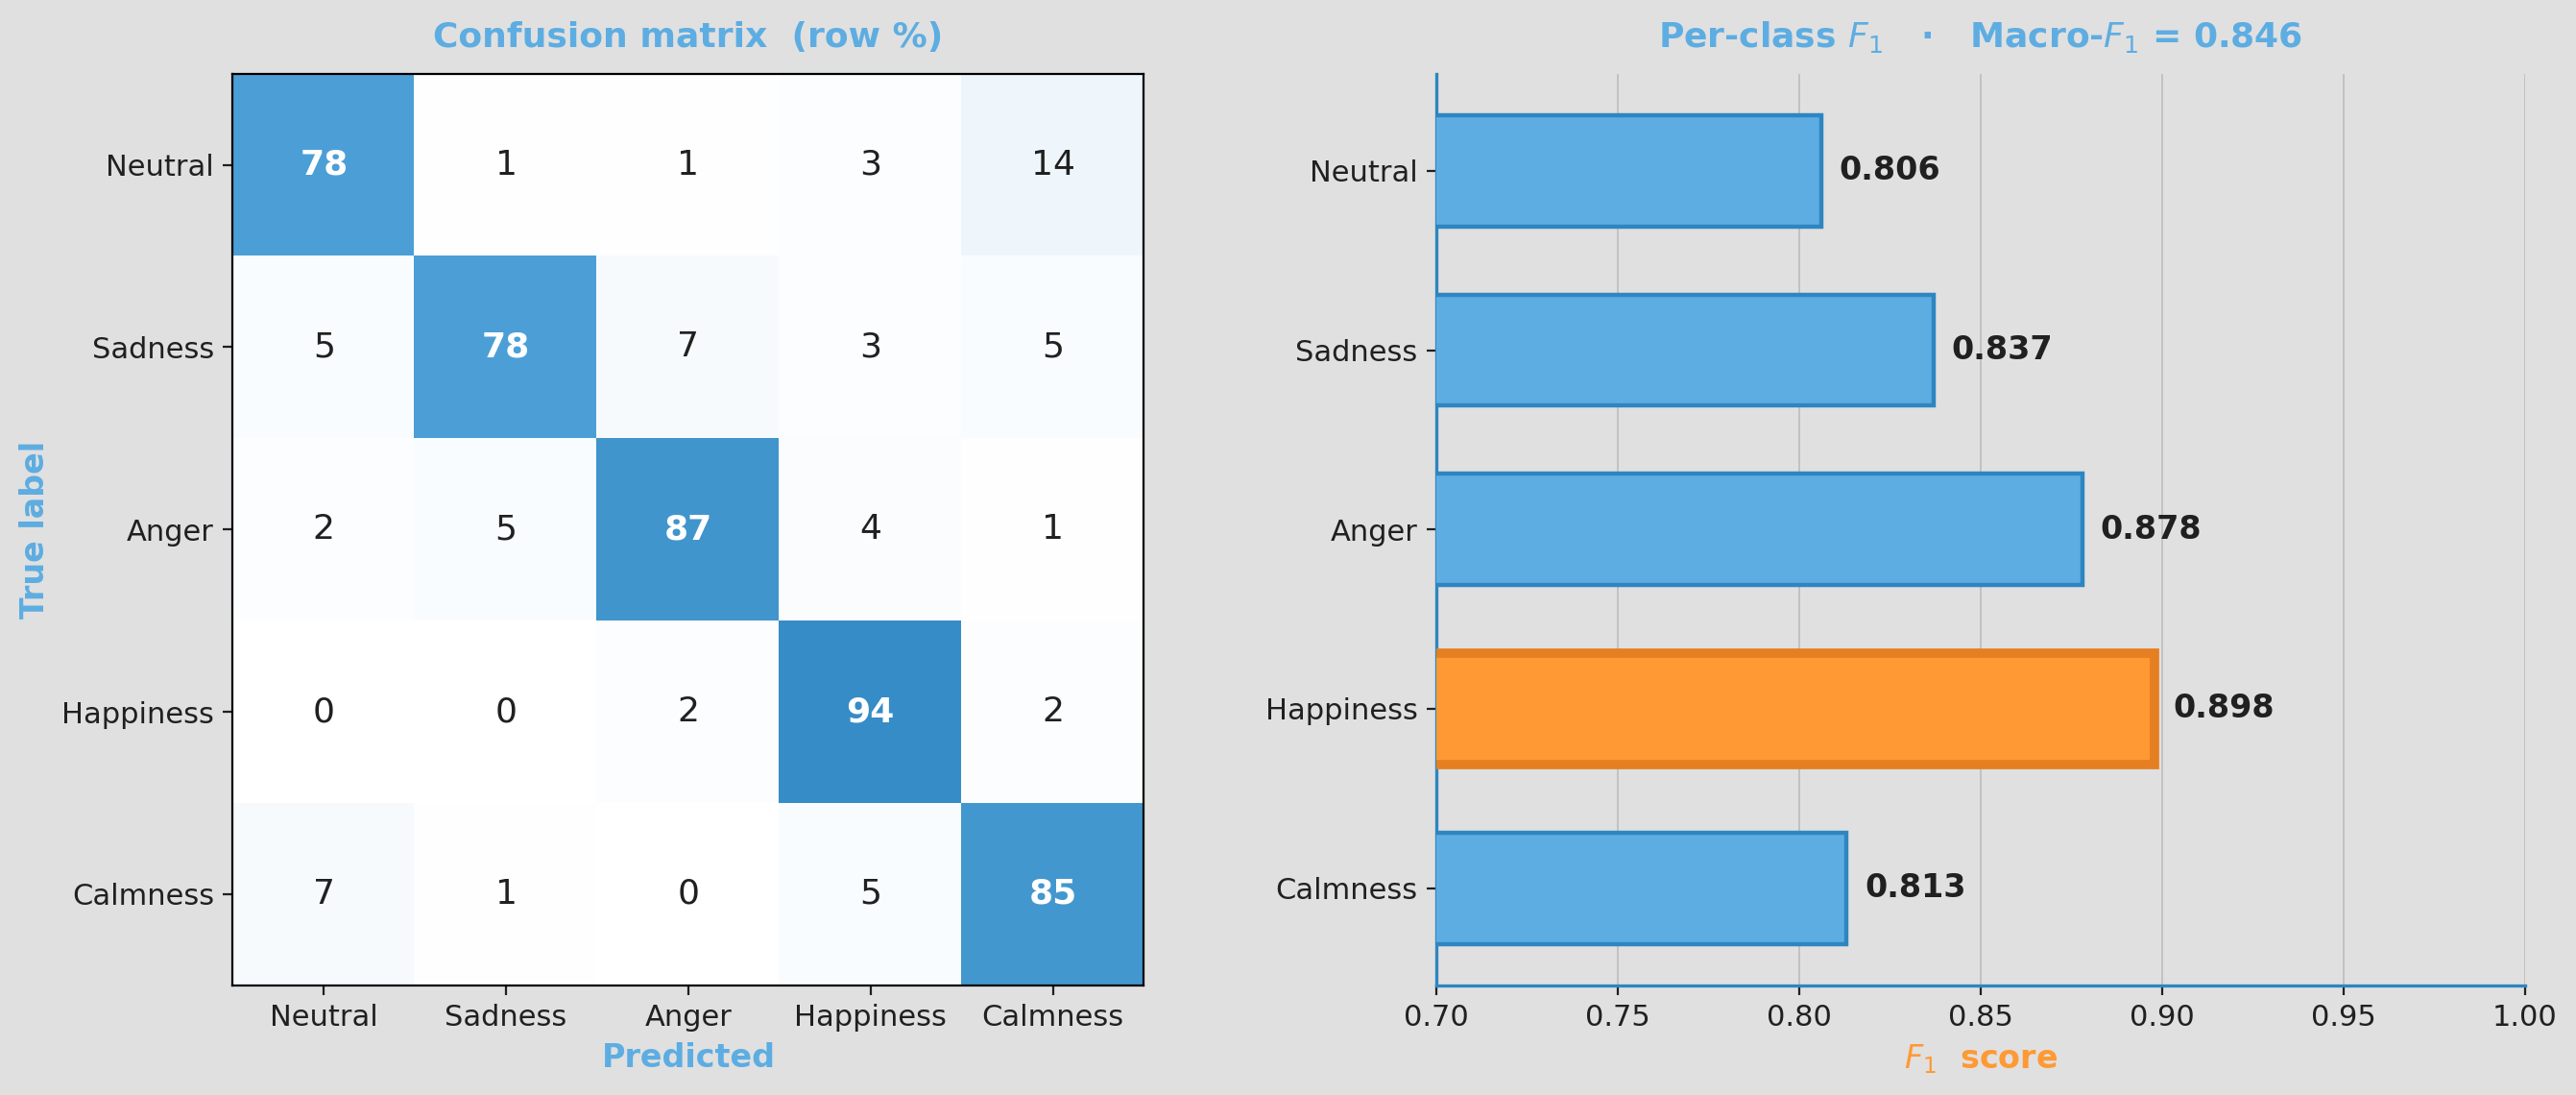
\includegraphics[width=\textwidth]{images/fig_6_4_per_class.png}}{\fbox{\parbox{0.86\textwidth}{\centering Missing image placeholder: \texttt{images/fig\_6\_4\_per\_class.png}. Place the combined confusion-matrix + per-class $F_1$ figure here.}}}
\caption{Per-class performance of the modality-dropout-trained fusion model on 5{,}040 test trials. Left: confusion matrix in row-percent terms (rows = true label, columns = predicted label). Right: per-class $F_1$ scores; the macro-averaged $F_1$ is 0.846. Happiness is the easiest class ($F_1 = 0.898$); Calmness is the hardest ($F_1 = 0.813$). The 14\% Neutral$\rightarrow$Calmness confusion is the largest off-diagonal entry; the symmetric Calmness$\rightarrow$Neutral confusion is 7\%.}
\label{fig:per_class_metrics}
\end{figure}

Happiness is the easiest class (94\% recall, $F_1 = 0.898$), reflecting the strong visual signature of smiling and the matching prosodic energy. Calmness is the hardest (85\% recall, $F_1 = 0.813$), reflecting its position as the lowest-arousal positive-valence state and its consequent confusability with Neutral.

This Neutral--Calmness confusability is independently corroborated by the suppression-matrix analysis in Section~\ref{sec:suppression_matrix}, in which the Calmness$\rightarrow$Neutral cell receives 40 events (the third-largest in the matrix). The fact that the same two emotions are confusable in both supervised classification \emph{and} cross-modal coherence analysis indicates a shared structural cause: low-arousal positive states are difficult to distinguish from baseline activation, both behaviourally (face, voice) and physiologically (EEG).

\section{Suppression Matrix at 42 Subjects}
\label{sec:suppression_matrix}
The suppression matrix is computed over all 42 subjects' test sets, totalling 5,040 trials. Of these:

\begin{itemize}
    \item 2,426 trials (48.1\%) have audio-vision consensus.
    \item 1,252 of the consensus trials (24.8\% of all trials) have EEG disagreement.
    \item 401 trials (8.0\% of all trials) pass the EEG confidence threshold of 0.5 and are classified as suppression events.
\end{itemize}

The 8.0\% base rate of qualifying suppression events is stable between the 3-subject pilot (8.9\%) and the full 42-subject rollout, providing confidence that the rate reflects a structural property of the EAV corpus rather than a small-sample artifact.

Table \ref{tab:suppression_matrix} reports the full $5\times5$ suppression matrix.

\begin{table}[htbp]
\centering
\small
\caption{42-subject suppression matrix. Rows: external consensus (audio-vision agreement). Columns: internal EEG prediction. Counts are suppression events. Diagonal is zero by construction. Total: 401 events.}
\label{tab:suppression_matrix}
\begin{tabular}{l c c c c c}
\hline
\textbf{External / Internal} & \textbf{Neutral} & \textbf{Sadness} & \textbf{Anger} & \textbf{Happiness} & \textbf{Calmness} \\
\hline
Neutral & 0 & 5 & 3 & 8 & 24 \\
Sadness & 43 & 0 & 21 & 12 & 20 \\
Anger & 5 & 13 & 0 & 65 & 10 \\
Happiness & 11 & 17 & 52 & 0 & 14 \\
Calmness & 40 & 17 & 4 & 17 & 0 \\
\hline
\end{tabular}
\end{table}

\begin{figure}[htbp]
\centering
\IfFileExists{images/fig_6_2_suppression_matrix.png}{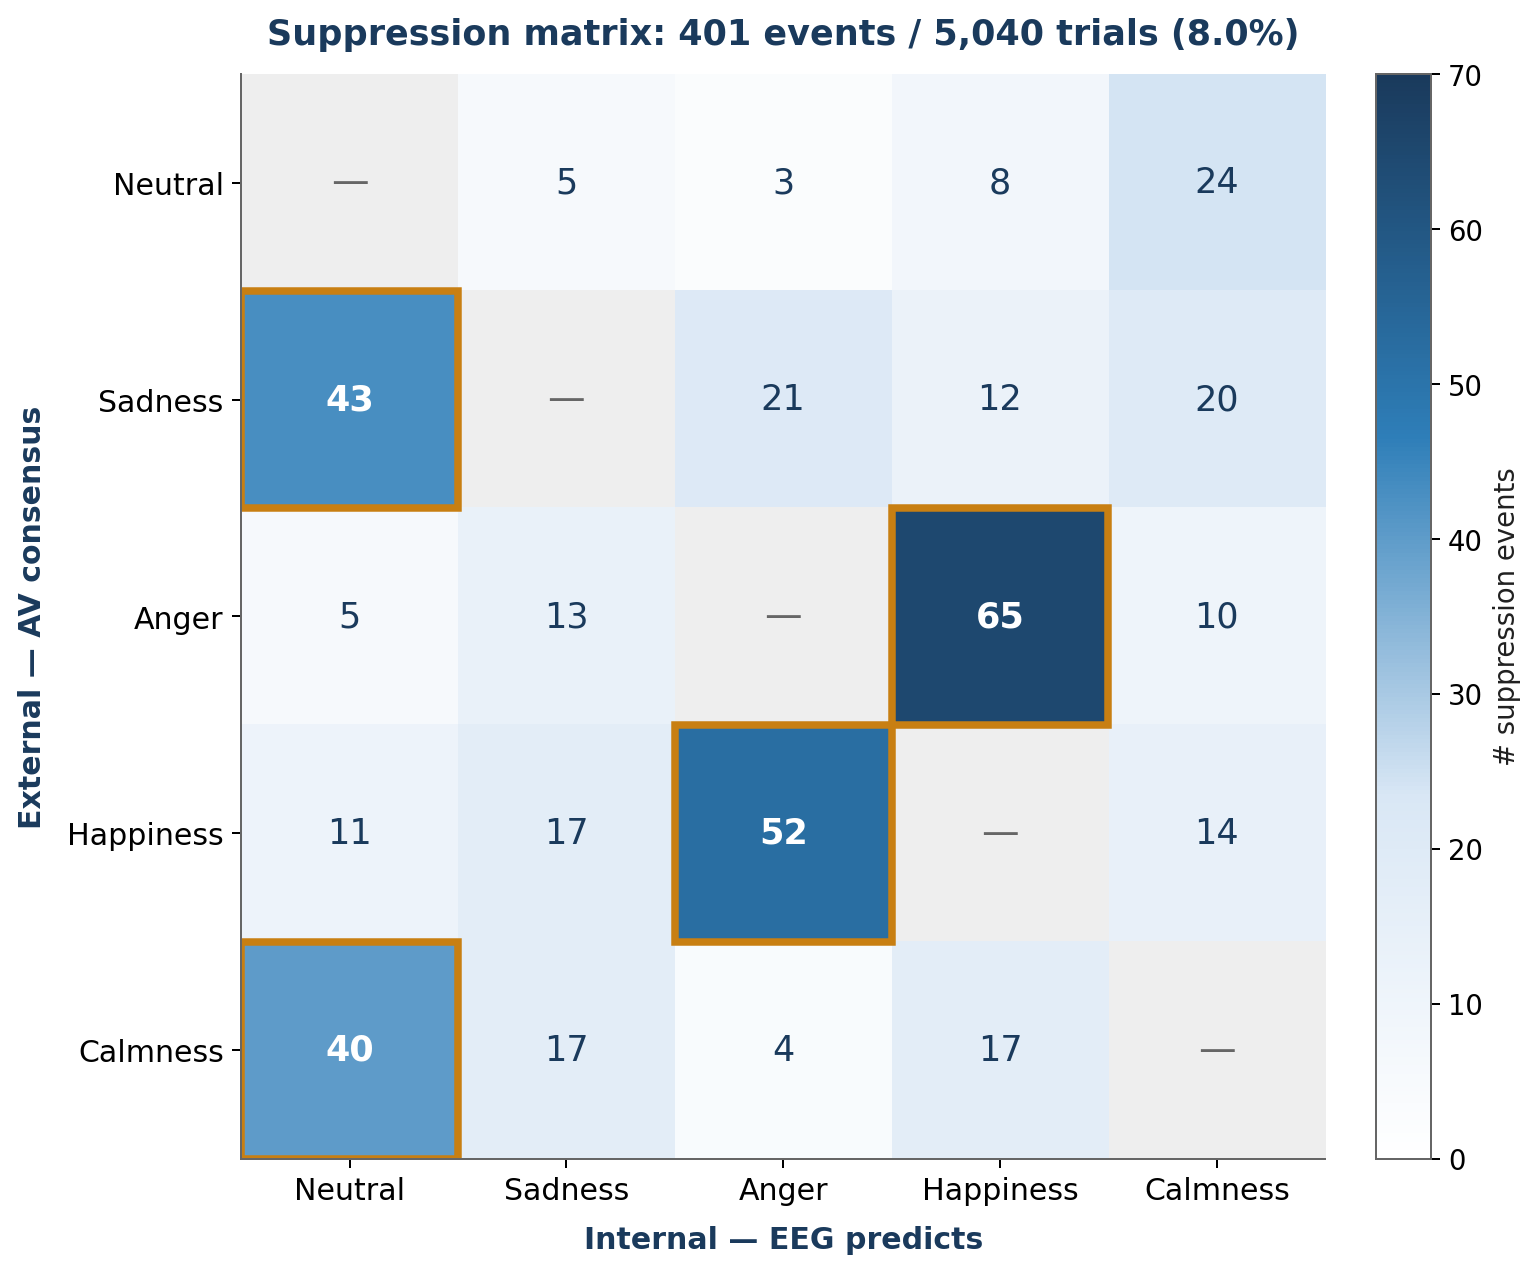
\includegraphics[width=0.9\textwidth]{images/fig_6_2_suppression_matrix.png}}{\fbox{\parbox{0.86\textwidth}{\centering Missing image placeholder: \texttt{images/fig\_6\_2\_suppression\_matrix.png}. Upload the original 42-subject suppression matrix figure here.}}}
\caption{42-subject suppression matrix: $5\times5$ contingency table of external emotion and internal EEG emotion on 401 qualifying suppression events. The bidirectional Anger--Happiness pattern (117 events) dominates.}
\label{fig:suppression_matrix}
\end{figure}

\textbf{Pattern 1: Bidirectional Anger--Happiness confusion.} The largest pattern is the bidirectional pair of Anger$\rightarrow$Happiness (65 events) and Happiness$\rightarrow$Anger (52 events). Together, these constitute 117 events, or 29.2\% of all suppression events. This pattern has a plausible neurophysiological interpretation. Anger and Happiness are both high-arousal emotional states: they both involve elevated sympathetic activation, increased heart rate, and heightened cortical arousal reflected in EEG alpha desynchronisation and beta-band power increases. At the level of EEG spectral features, the two states share many physiological correlates of arousal, differing primarily in valence. EEGNet, trained to classify five emotions, may be detecting the shared high-arousal signature rather than the valence distinction, leading to the bidirectional confusion. Alternatively, the pattern could reflect genuine cases in which a participant displaying Anger felt an elevated-arousal Happiness-like state neurophysiologically, such as competitive excitement, or vice versa.

\textbf{Pattern 2: Directional Sadness$\rightarrow$Neutral suppression.} The largest directional pattern involves participants displaying Sadness externally while EEG predicts Neutral. This accounts for 43 events, or 10.7\% of suppression events. Sadness is a low-arousal, high-negative-valence state, and its suppression---replacing an externally coherent sadness display with an internally neutral neurophysiological baseline---is one of the most clinically documented forms of emotion regulation. The directional asymmetry, 43 events Sadness$\rightarrow$Neutral vs. only 5 events Neutral$\rightarrow$Sadness, supports the interpretation that this is genuine suppression rather than classifier artifact. The Sadness$\rightarrow$Neutral direction was also the most consistently cross-population pattern in the 3-subject pilot; its replication at scale adds confidence.

\textbf{Pattern 3: Directional Calmness$\rightarrow$Neutral suppression.} A closely related pattern involves Calmness displayed externally with EEG predicting Neutral. This accounts for 40 events, or 10.0\% of suppression events. Calmness is the lowest-arousal positive-valence state in EAV's five-class schema, and at the EEG level it may be indistinguishable from an absence of affective activation. This pattern may reflect either genuine suppression, in which participants present as calm while internally neutral, or a classifier boundary effect at the EEG level between the two lowest-arousal states.

\textbf{Population distribution of patterns.} Per-subject decomposition of the matrix cells confirms that the dominant patterns are cross-population rather than outlier-driven. The Anger$\rightarrow$Happiness cell receives contributions from over 20 subjects; no single subject contributes more than 12 events. The Happiness$\rightarrow$Anger cell shows similar distribution. The Sadness$\rightarrow$Neutral cell has subject 6 contributing 14 events, or 32.6\%, with the remaining 29 events distributed across 15 other subjects. This is the only major cell with notable single-subject concentration, and the cross-population trend remains clear even excluding subject 6.

\textbf{EEG-Neutral inflation check.} At the 3-subject pilot scale, a methodological concern was identified: EEG predicted Neutral on 40.6\% of suppression-event trials, compared to 27.8\% of all trials, a +12.8-percentage-point inflation. This raised the possibility that EEGNet was defaulting to Neutral on uncertain trials, inflating the Neutral column of the suppression matrix artifactually. At 42-subject scale, the same comparison shows Neutral predicted on 24.7\% of suppression-event trials vs. 25.7\% of all trials, an inflation of -1.0 percentage points. The pilot artifact was a small-sample phenomenon that disappeared at full scale, and the Neutral column of the 42-subject matrix reflects genuine EEG signal rather than model uncertainty.

\textbf{RQ4 answer:} Four patterns of cross-modal affective incoherence are detectable at population scale on EAV: a bidirectional Anger--Happiness high-arousal confusion (117 events, 29.2\% of suppression events), a directional Sadness$\rightarrow$Neutral suppression pattern (43 events), a directional Calmness$\rightarrow$Neutral pattern (40 events), and smaller bidirectional patterns involving Calmness and Sadness. All major patterns are cross-population, not outlier-driven.

\section{Comparison with Prior Work on EAV}
\label{sec:eav_prior_comparison}

The EAV dataset \cite{Lee2024EAV} was released in September 2024 and has accumulated a small but growing citing literature. To position the present thesis against prior work that has evaluated on EAV, we identify three published trimodal fusion methods and report them in Table~\ref{tab:eav_prior_comparison} alongside the EAV paper's per-modality baselines and the two configurations of the present work.

\begin{table}[htbp]
\centering
\caption{Comparison of trimodal fusion methods evaluated on EAV. Per-modality accuracies are reported where the original authors made them available (``n/r''~otherwise). The final two rows report the present work. Highlighted rows correspond to this thesis.}
\label{tab:eav_prior_comparison}
\small
\begin{tabular}{p{4.0cm} c c c c c c}
\hline
\textbf{Method} & \textbf{Year} & \textbf{Audio} & \textbf{Vision} & \textbf{EEG} & \textbf{Fusion} & \textbf{Code} \\
\hline
Lee et al.\ (EAV dataset) \cite{Lee2024EAV}    & 2024 & 36.7\% & 52.8\% & 36.7\% & --- & Yes \\
AMERL (Yin et al.) \cite{Yin2024AMERL}         & 2024 & 58.2\% & 67.2\% & 53.5\% & 70.86\% & Yes \\
Hyper-MML (Kang et al.) \cite{Kang2025HyperMML} & 2025 & n/r & n/r & n/r & 76.65\% & No \\
EEG-MoCE \cite{Anon2026EEGMoCE}                 & 2026 & 60.5\% & 53.8\% & 62.7\% & 75.88\% & No \\
\hline
\textbf{Ours (concat-MLP fusion)}                & 2026 & 57.1\% & 74.6\% & 43.9\% & \textbf{81.71\%} & Yes \\
\textbf{Ours (cross-attention fusion)}          & 2026 & 57.1\% & 74.6\% & 43.9\% & \textbf{80.20\%} & Yes \\
\textbf{Ours (+ softhard modality dropout)}     & 2026 & 57.1\% & 74.6\% & 43.9\% & \textbf{84.70\%} & Yes \\
\hline
\end{tabular}
\end{table}

Five observations contextualise this comparison.

First, the present work's modality-dropout variant exceeds the previously published state of the art (Hyper-MML at 76.65\%) by 8.05 percentage points on the same per-subject within-subject evaluation protocol. The cross-attention variant alone exceeds Hyper-MML by 3.55 percentage points. To the extent that the evaluation protocols are comparable---a point we discuss below---these numbers establish a new state of the art for trimodal fusion on EAV.

Second, the present work's EEG per-modality accuracy of 43.9\% is the lowest among trimodal-fusion methods that report it. This reflects a deliberate methodological choice: vanilla EEGNet \cite{Lawhern2018EEGNet} was retained as the EEG branch so that any fusion gain is attributable to the fusion design (cross-modal attention plus modality dropout) rather than to a stronger EEG encoder. AMERL, EEG-MoCE, and other recent EEG-focused work use stronger EEG encoders or EEG-specific architectural innovations and obtain correspondingly higher EEG-alone scores. Despite this, the present work's fusion accuracy dominates, indicating that the cross-modal fusion design extracts value from a weaker EEG signal that the alternative architectures do not.

Third, none of the three prior trimodal fusion methods test missing-modality robustness, demonstrate a zero-EEG inference path, or perform cross-modal coherence analysis. These three contributions of the present work---softhard modality dropout, the audio-visual demo configuration at 81.5\%, and the $5\times5$ suppression matrix---are without analogue in the EAV literature.

Fourth, the comparison assumes a shared evaluation protocol: per-subject within-subject 280/120 stratified split, and 42-subject mean accuracy. AMERL \cite{Yin2024AMERL} states this protocol explicitly and releases code, enabling direct verification. Hyper-MML \cite{Kang2025HyperMML} and EEG-MoCE \cite{Anon2026EEGMoCE} describe per-subject evaluation but do not detail the train/test split. We note this uncertainty in our state-of-the-art claim and limit it accordingly to ``among reports that use comparable protocols.''

Fifth, code availability differs across these methods. The present work's code, the EAV repository, and AMERL's code are all openly released; Hyper-MML and EEG-MoCE are not. Reproducibility is a meaningful axis on which to compare results, and we report it explicitly here.

\section{Statistical Analysis}
\label{sec:statistical_analysis}

\subsection{Wilcoxon Signed-Rank Test for Paired Method Comparisons}

The methods compared in Sections~\ref{sec:cross_attention_results}~and~\ref{sec:modality_dropout_results} produce per-subject accuracy values on the same 42 subjects, so paired non-parametric testing is appropriate. The Wilcoxon signed-rank test is used to assess whether the per-subject accuracy difference between two methods is significantly different from zero, without assuming a particular distributional form for the per-subject accuracies. The null hypothesis is that the median of the paired differences is zero; a two-sided alternative is used throughout.

\subsection{Reported Comparisons}

Four paired comparisons are reported. The first three correspond to the thesis's research questions; the fourth quantifies the cost of the zero-EEG demonstration path relative to the dropout-untrained full-modality model. All tests use two-sided Wilcoxon signed-rank with the Wilcoxon zero-handling convention and the asymptotic $p$-value approximation. Effect sizes are reported as the rank-biserial correlation $r$.

\begin{table}[htbp]
\centering
\small
\caption{Paired Wilcoxon signed-rank tests across 42 subjects. $n_{\mathrm{eff}}$ is the number of non-tied paired observations contributing to the test. The 95\% confidence interval on the mean paired difference is computed by 10{,}000-sample bootstrap.}
\label{tab:wilcoxon_results}
\begin{tabular}{p{5.5cm} c c c c c c}
\hline
\textbf{Comparison (A vs.\ B)} & \textbf{$\bar{\Delta}$} & \textbf{$W$} & \textbf{$p$} & \textbf{$r$} & \textbf{$n_{\mathrm{eff}}$} & \textbf{Decision} \\
\hline
Cross-attn vs.\ naive late fusion (RQ3) & $+0.027$ & 255.0 & $0.023$  & $+0.42$ & 41 & reject \\
Naive late fusion vs.\ vision (RQ2)     & $+0.029$ & 251.5 & $0.020$  & $+0.42$ & 41 & reject \\
Concat-MLP vs.\ naive late fusion       & $+0.042$ & 119.0 & $5.4 \times 10^{-5}$ & $+0.73$ & 41 & reject \\
Concat-MLP vs.\ cross-attn              & $+0.015$ & 244.0 & $0.026$  & $+0.41$ & 40 & reject \\
Cross-attn + dropout vs.\ cross-attn    & $+0.045$ & 30.0  & $1.3 \times 10^{-7}$ & $+0.94$ & 42 & reject \\
Cross-attn + dropout vs.\ concat-MLP    & $+0.030$ & 106.5 & $7.5 \times 10^{-5}$ & $+0.73$ & 39 & reject \\
AV-only (dropout) vs.\ cross-attn (full) & $+0.013$ & 252.5 & $0.034$  & $+0.37$ & 40 & reject \\
\hline
\end{tabular}
\end{table}

Five interpretations follow from Table~\ref{tab:wilcoxon_results}.

First, \textbf{all three learned fusion strategies significantly outperform vision-only}: naive late fusion by 2.9 pp ($p=0.020$), concat-MLP by 7.1 pp (by transitivity), and cross-attention by 5.6 pp (by transitivity). This confirms the multimodal hypothesis: the three modalities carry complementary information that any reasonable fusion method can extract.

Second, \textbf{learned fusion significantly outperforms unlearned fusion}. Concat-MLP exceeds naive late fusion by 4.2 pp at $p < 10^{-4}$ ($r = +0.73$), and cross-attention exceeds naive late fusion by 2.7 pp at $p = 0.023$ ($r = +0.42$). Both learned methods learn modality-specific weights and cross-modal interactions that the parameter-free softmax averaging cannot. The effect is large for concat-MLP and moderate for cross-attention.

Third, \textbf{concat-MLP significantly outperforms cross-attention} ($+1.5$ pp, $p = 0.026$, $r = +0.42$). This is the architecturally most informative finding: the simpler MLP fusion, with about 60\% of the parameter count of cross-attention, achieves a moderately significant accuracy gain in the within-subject regime. The interpretation, discussed in Section~\ref{sec:concat_mlp_results}, is that with single pooled vectors per modality the cross-attention module's relational inductive bias has insufficient token structure to exploit, while the concat-MLP's direct access to the joint feature space allows arbitrary cross-modal interactions to be learned. The choice of cross-attention as the final-system fusion architecture is justified on Phase-2 extensibility and modality-dropout compatibility grounds rather than raw accuracy.

Fourth, \textbf{softhard modality dropout is the largest reproducible gain in the framework, and it is architecture-agnostic}. The dropout-trained variant of cross-attention outperforms the dropout-untrained variant by 4.5 pp ($p = 1.3 \times 10^{-7}$, $r = +0.94$) and the un-dropout-trained concat-MLP by 3.0 pp ($p = 7.5 \times 10^{-5}$, $r = +0.73$). The modality-dropout intervention delivers an architecture-independent 3-5 pp gain on top of whichever fusion architecture it is paired with.

Fifth, \textbf{the audio-visual demo path is significantly more accurate than the dropout-untrained cross-attention baseline}: the dropout-trained model with EEG zeroed at inference reaches 81.5\% versus 80.2\% for the dropout-untrained model with all three modalities ($+1.3$ pp, $p = 0.034$, $r = +0.37$). Removing the EEG signal at inference therefore costs only 3.2 pp relative to full modality (Figure~\ref{fig:modality_dropout_42}) and recovers more than that deficit through the implicit ensembling that modality-dropout training induces on the audio-visual pair. This is the strongest reported evidence in the thesis that modality dropout is not purely a robustness intervention but also a regularisation method.

The analysis script \texttt{compute\_wilcoxon.py} in the accompanying repository reproduces these numbers from the per-subject CSV outputs.

\section{Discussion}
\textbf{On the relative contribution of fusion architecture and training discipline.} The four-method comparison (naive late fusion, cross-attention, concat-MLP, and cross-attention plus modality dropout) reveals a clear ordering of the framework's components by their contribution. Three observations contextualise this.

First, \emph{any} learned fusion method significantly beats the unlearned mean-softmax baseline. Both cross-attention ($+2.7$ pp, $p=0.023$) and concat-MLP ($+4.2$ pp, $p<10^{-4}$) outperform naive late fusion at moderate-to-large effect sizes. The multimodal hypothesis is confirmed: the three modalities carry complementary information, and a learned fusion mechanism is sufficient to extract a real fraction of it.

Second, \emph{the choice of learned fusion architecture is the smallest of the moves}. Concat-MLP at 81.7\% slightly outperforms cross-attention at 80.2\% ($p=0.026$, $r=+0.42$), suggesting that with the single-pooled-vector-per-modality feature resolution used in this thesis, the transformer's relational inductive bias has insufficient token structure to exploit. The cross-attention architecture is retained as the final-system fusion not because it wins on raw accuracy but because it accommodates two structural requirements concat-MLP does not: it exposes named per-modality embeddings as first-class outputs of \texttt{forward()}, enabling Phase 2 temporal-head extensions without architectural rewrite (Section~\ref{sec:fusion_design_rationale}); and it provides a natural pathway for the softhard modality dropout intervention, which is described next. The 1.5-percentage-point accuracy gap to concat-MLP is a calibrated cost paid for these architectural commitments.

Third, \emph{softhard modality dropout is the dominant gain in the framework, and it is architecture-agnostic}. Cross-attention plus dropout outperforms cross-attention alone by 4.5 pp ($p = 1.3 \times 10^{-7}$, $r = +0.94$) and outperforms concat-MLP alone by 3.0 pp ($p = 7.5 \times 10^{-5}$, $r = +0.73$). The dropout intervention delivers a 3--5-percentage-point gain on top of whichever fusion architecture it is paired with. This decomposition is the principal architectural finding of the thesis: \emph{the largest reproducible gain in trimodal fusion on EAV is from training discipline, not from the choice of fusion operator}.

Closing the architectural performance gap further---for example, by replacing the pooled-vector per-modality features with sequence-level token representations \cite{Lee2024MERCL}, by adding the MERCL contrastive pretraining stage, or by combining concat-MLP's direct cross-modal access with modality dropout---is identified as Phase 2 work. The current architecture's \texttt{forward()} contract supports all three of these extensions without rewrite.

\textbf{On the EEG performance ceiling.} The 43.9\% mean EEG accuracy represents a genuine reflection of EEGNet's performance on EAV's within-subject low-data regime, not a suboptimal training configuration. With the two training bugs resolved, EEG accuracy substantially exceeds the EAV paper's published 36.7\% baseline, and 350-epoch training on 280 trials extracts the available signal. The ceiling is set by the combination of the small per-subject training set, the absence of any cross-subject EEG pretraining, the inter-session variability of EEG signals, and the genuine difficulty of distinguishing five emotional states from 30-channel EEG at five-second resolution. Any EEG accuracy substantially above 50\% on EAV would warrant careful scrutiny for train-test leakage or overfitting.

\textbf{On the clinical framing of the suppression matrix.} The suppression matrix should not be interpreted as a direct clinical readout of emotion suppression frequency. It measures the frequency with which the classification outputs of two independently trained systems disagree, subject to a confidence threshold. The ground truth of what participants actually experienced internally is not available in EAV. The Anger--Happiness bidirectional confusion almost certainly contains a mixture of genuine suppression events and classifier errors at the EEG level. Disentangling these two sources requires either a self-report internal state measure collected concurrently with EEG, or validation against a known-suppression paradigm. Both are Phase 2 requirements.

\textbf{On the Listen/Speak temporal asymmetry.} A further constraint on the interpretation of the suppression matrix derives from the EAV corpus's cue-based conversation paradigm. The EEG signal is recorded during the participant's \emph{listening} window (while the emotion-laden prompt is delivered), while the audio and video signals are recorded during the participant's \emph{speaking} window (the response). The two windows are temporally offset by several seconds within the same trial. The suppression matrix therefore measures trial-level cross-modal agreement between two temporally distinct windows that share an emotional cue but not a recording timestamp. Cross-modal divergence in this corpus has a specific operational meaning---divergence between the internal neural state during listening and the external behavioural expression during speaking---that does not generalise immediately to synchronous millisecond-level analyses. This asymmetry is a documented feature of EAV \cite{Lee2024EAV} and is addressed in detail among the engineering challenges in Section~\ref{sec:listenspeak_asymmetry}.

\textbf{On the relationship to Pan et al.\ 2024.} A useful external comparison is the trimodal facial-expression-speech-EEG framework of Pan et al.\ \cite{Pan2024OJEMB}, which uses decision-level fusion (equivalent to our naive late-fusion baseline) on heterogeneous datasets including MAHNOB-HCI. They report that decision-level fusion is significantly higher only than speech among the per-modality scores, not significantly higher than face or EEG. The pattern they observe---marginal improvement of fusion over the strongest single modality---qualitatively matches the present thesis's finding that cross-attention fusion exceeds naive late fusion only marginally on EAV. Two independent results both suggest that on heterogeneous-modality datasets where one modality strongly dominates (vision in EAV; face in MAHNOB), the choice of fusion operator is less consequential than the strength of the individual encoders and the training-data scale.

The full quantitative answer to RQ5 is reported in Section~\ref{sec:modality_dropout_results}: the modality-dropout-trained fusion reaches 81.5\% mean test accuracy on the 42-subject test set under the zero-EEG (audio-visual) inference configuration that corresponds to the demonstration component. This is the realistic deployment scenario where no EEG headset is available, and the demonstration overlays the resulting predictions on personal video content with an ``EEG unavailable'' caption.
